\chapter{Participation statistics}
\label{app:participation}

\section{Descriptives}

\begin{longtable}[c]{@{}lrrrrrrrrrr@{}}
    \caption{Including users with no active days}
\endfirsthead
\toprule\addlinespace
& N & min & max & mean & var & skew & kurt & normal-t & normal-p
\\\addlinespace
\midrule
\textbf{Flashcards} & 33 & 0 & 7 & 3.27 & 7.58 & 0.02 & -1.75 & 56.992 &
0.0000
\\\addlinespace
\textbf{Flashmap} & 30 & 0 & 11 & 3.27 & 10.41 & 0.39 & -1.04 & 3.868 &
0.1446
\\\addlinespace
\textbf{General} & 63 & 0 & 11 & 3.27 & 8.78 & 0.24 & -1.26 & 22.212 &
0.0000
\\\addlinespace
\bottomrule
    \label{tab:participation_incl}
\end{longtable}

\begin{longtable}[c]{@{}lrrrrrrrrrr@{}}
    \caption{Excluding users with no active days}
\endfirsthead
\toprule\addlinespace
& N & min & max & mean & var & skew & kurt & normal-t & normal-p
\\\addlinespace
\midrule
\textbf{Flashcards} & 25 & 1 & 7 & 4.32 & 5.39 & -0.48 & -1.47 & 11.919
& 0.0026
\\\addlinespace
\textbf{Flashmap} & 19 & 1 & 11 & 5.16 & 6.47 & -0.12 & 0.11 & 0.624 &
0.7321
\\\addlinespace
\textbf{General} & 44 & 1 & 11 & 4.68 & 5.90 & -0.24 & -0.50 & 0.823 &
0.6628
\\\addlinespace
\bottomrule
    \label{tab:participation_excl}
\end{longtable}

\FloatBarrier
\section{Comparisons among conditions}

\begin{longtable}[c]{@{}lrrrr@{}}
\toprule\addlinespace
& \textbf{Mann-Whitney-U k} & \textbf{Mann-Whitney-U p} &
\textbf{Welch's t-test k} & \textbf{Welch's t-test p}
\\\addlinespace
\midrule\endhead
& 0.008 & 0.9936 & 0.008 & 0.9937
\\\addlinespace
\bottomrule
    \label{tab:participation-comp}
\end{longtable}

\begin{figure}[htbp]
    \centering
    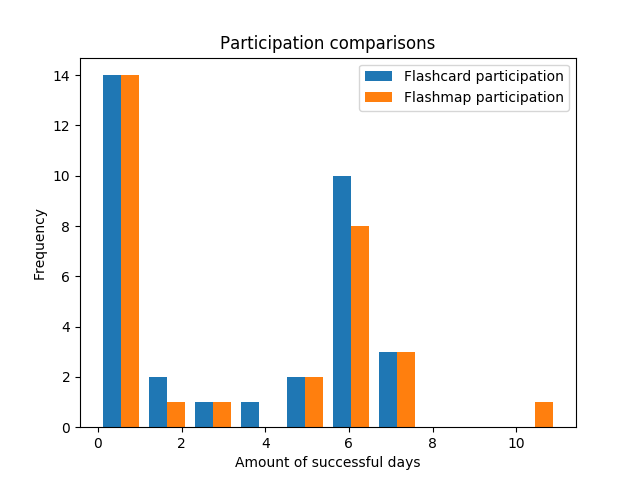
\includegraphics[width=.7\textwidth]{img/participation.png}
    \caption{A histogram comparing the amount of active days between flashcard and flashmap users}
    \label{fig:participation}
\end{figure}
\begin{figure}
    \centering
    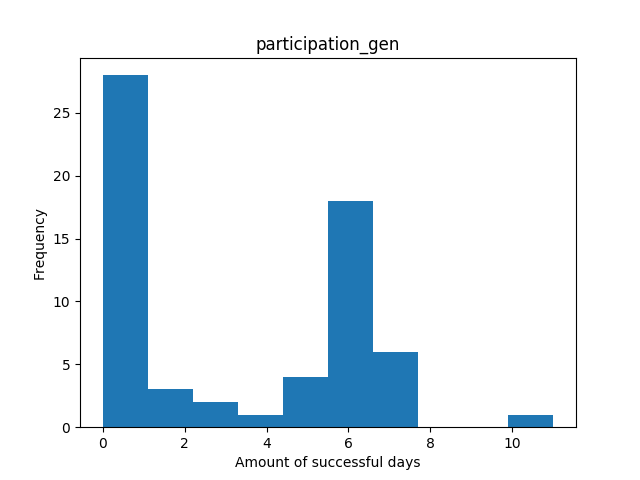
\includegraphics[width=.7\textwidth]{img/participation_gen.png}
    \caption{A histogram depicting the amount of active days of all participants}
    \label{fig:participation_gen}
\end{figure}
\begin{figure}
    \centering
    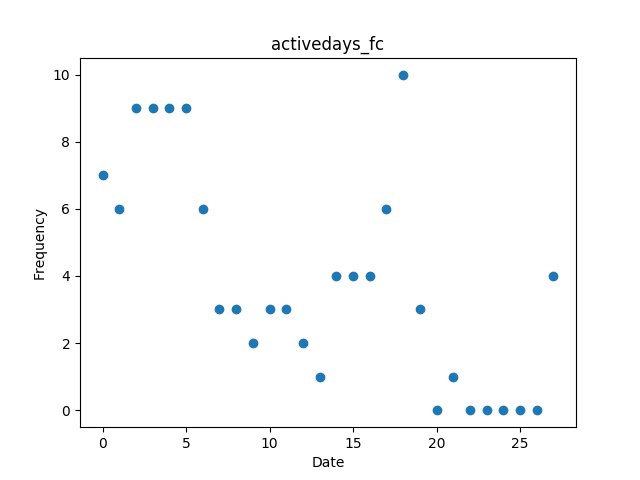
\includegraphics[width=.7\textwidth]{img/activedays_fc.png}
    \caption{A scatter diagram depicting how many flashcard users were active during which day of the experiment, combined with a step diagram depicting how many flashcard users finished the experiment that day (more than or equal to 6 successful days)}
    \label{fig:activedays_fc}
\end{figure}
\begin{figure}
    \centering
    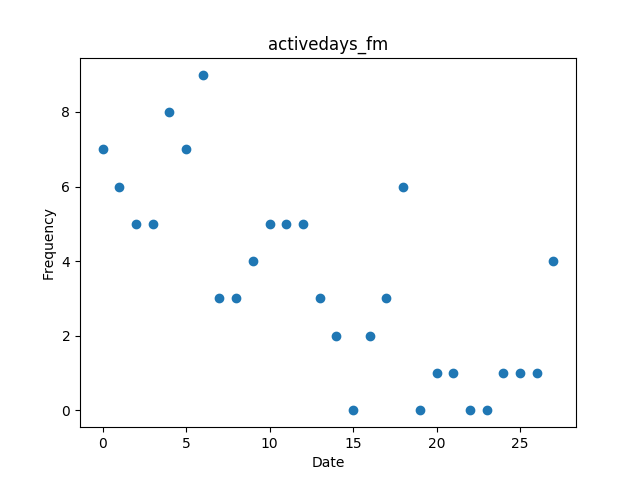
\includegraphics[width=.7\textwidth]{img/activedays_fm.png}
    \caption{A scatter diagram depicting how many flashmap users were active during which day of the experiment, combined with a step diagram depicting how many flashmap users finished the experiment that day (more than or equal to 6 successful days)}
    \label{fig:activedays_fm}
\end{figure}
